\documentclass{report}
\usepackage[utf8]{inputenc}
\usepackage{graphicx}
\usepackage{algorithm2e}
\usepackage{minted}
\usepackage{xcolor}
\usepackage{biblatex}
\usepackage{hyperref}
\addbibresource{210050037_outlab4.bib}
\begin{document}
\begin{titlepage}
\begin{center} 

\vspace*{6.85cm}

{\bfseries \huge Software Systems Lab: Outlab}

\vspace{1cm}

{\bfseries \huge \LaTeX}

\vspace{1cm}

{\Large Name: BVSS Prabandh}

\vspace{0cm}

{\Large Roll\_no: 210050037}

\vspace{1cm}

{\Large August 30,2022}
\end{center}
\end{titlepage}
\tableofcontents
\newpage
\chapter{\Large Introduction}
\section{\large Dictionary}
   
In this report we would see different algorithms for dictionary ADTS.We would calculate big-oh notations for all algorithms and find the efficient.

\vspace{1cm}

Dictionary\cite{1} (map, association list) is a data structure, which is generally an association of unique keys with some values. One may bind a value to a key, delete a key (and naturally an associated value) and lookup for a value by the key. Values are not required to be unique. Simple usage example is an explanatory dictionary. In the example, words are keys and explanations are values.
Dictionary ADT

\vspace{1cm}

\textbf{\large Operations}

\vspace{0.5cm}

    Dictionary create()
    creates empty dictionary
    
\vspace{1cm}

    boolean isEmpty(Dictionary d)\\
    tells whether the dictionary d is empty
    
\vspace{0.5cm}

    put(Dictionary d, Key k, Value v)\\
    associates key k with a value v;
    if key k already presents in the dictionary
    old value is replaced by v
    
\vspace{0.5cm}

    Value get(Dictionary d, Key k)\\
    returns a value, associated with key k
    or null, if dictionary contains no such key
    
\vspace{0.5cm}

    remove(Dictionary d, Key k)\\
    removes key k and associated value
    destroy(Dictionary d)
    destroys dictionary d
\newpage
\chapter{\Large Sorted or Unsorted?}
The Question is do we want to store values in sorted of keys or unsorted.

\vspace{1cm}

Lets see pros and Cons

\vspace{1cm}

\textbf{\large SEARCH :} 
\vspace{1cm}

Sorted takes O(logn) while unsorted O(n\^2)

\vspace{1cm}

\textbf{\large INSERT :}

\vspace{1cm}

Sorted takes O(n) while unsorted O(1)

\vspace{1cm}

\textbf{\large DELETION :}

\vspace{1cm}

Sorted takes O(n) while unsorted O(n\^2)
\newpage
\chapter{\Large Different Algorithms}
\Large Different Algorithms:
\begin{enumerate}
    \item \large Hashing
    \begin{itemize}
            \item hash function
            \item good hash function ?
            \item chaining
            \item probing
        \end{itemize}
    \item \large BST
\end{enumerate}
\section{\large Hashing}
Hashing\cite{2} uses functions or algorithms to map object data to a representative integer value. A hash can then be used to narrow down searches when locating these items on that object data map.

For example, in hash tables, developers store data -- perhaps a customer record -- in the form of key and value pairs. The key helps identify the data and operates as an input to the hashing function, while the hash code or the integer is then mapped to a fixed size.

Hash tables support functions that include the following: \\
\\
insert (key, value) \\
get (key) \\
delete (key) \\
\subsection{\large Hashfunction}
A function that converts a given big phone number to a small practical integer value. The mapped integer value is used as an index in the hash table. In simple terms, a hash function maps a big number or string to a small integer that can be used as the index in the hash table. 
\subsection{\large Good Hashfunction}
A good hash function should have the following properties: 
\begin{itemize}
    \item Efficiently computable.
    \item Should uniformly distribute the keys (Each table position equally likely for each key)
\end{itemize}
Hash tables have very different requirements. But still, finding a good hash function universally is hard because different data types expose different information that can be hashed. As a rule of thumb it is good to consider all information a type holds equally. This is not always easy or even possible. For reasons of statistics (and hence collision), it is also important to generate a good spread over the problem space, i.e. all possible objects. This means that when hashing numbers between 100 and 1050 it's no good to let the most significant digit play a big part in the hash because for ~ 90\% of the objects, this digit will be 0. It's far more important to let the last three digits determine the hash.
\subsection{\large How to resolve collisions ?}
\textbf{CHAINING:}\\
In the chaining approach, the hash table is an array of linked lists i.e., each index has its own linked list.
All key-value pairs mapping to the same index will be stored in the linked list of that index.
The benefits of chaining
\begin{itemize}
    \item Through chaining, insertion in a hash table always occurs in O(1) since linked lists allow insertion in constant time.

    \item Theoretically, a chained hash table can grow infinitely as long as there is enough space.

    \item A hash table which uses chaining will never need to be resized.

\end{itemize}
HASH TABLE: \\
\begin{center}
\begin{tabular}{|c|c|c|c|c|c|c|c|c|} 
 \hline
 array\_index & node1 & node2 & node3 & node4 & node5 & ....\\ [1ex]
 \hline\hline
 1 & 6 & 87837  \\ 
 \hline
 2 & 7 & 78 & 5415 & 1234 & 345\\
 \hline
 3 & 545 & 778 & 7507 \\
 \hline
 4 & 545 & 18744 & 7560 & 1278\\
 \hline
 5 & 88 \\ [1ex] 
 \hline
\end{tabular}
\end{center}
\newpage 
\textbf{PROBING:}\\
In linear probing\cite{3}, the hash table is searched sequentially that starts from the original location of the hash. If in case the location that we get is already occupied, then we check for the next location. 
The function used for rehashing is as follows: rehash(key) = (n+1)\%table-size.\\
If slot hash(x) \% S is full, then we try (hash(x) + 1) \% S\\
If (hash(x) + 1) \% S is also full, then we try (hash(x) + 2) \% S\\
If (hash(x) + 2) \% S is also full, then we try (hash(x) + 3) \% S \\
..................................................\\
..................................................\\
\begin{figure}[h]
\caption{Example of probing}

\vspace{0.5cm}
\centering
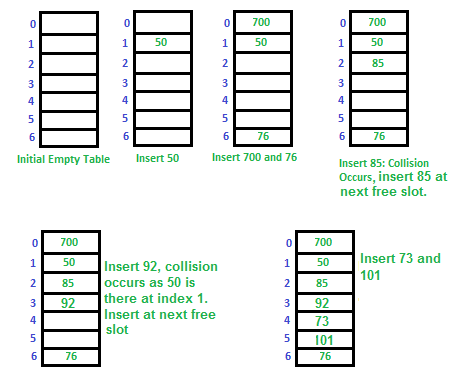
\includegraphics[width=0.5\textwidth]{probing.png}
\end{figure}
\newpage
\section{\large BST}
Binary Search Tree is a node-based binary tree data structure which has the following properties:
\begin{itemize}
    \item The left subtree of a node contains only nodes with keys lesser than the node’s key.
    \item The right subtree of a node contains only nodes with keys greater than the node’s key.
    \item The left and right subtree each must also be a binary search tree.
\end{itemize}
\begin{figure}[h]
\caption{Example of a BST}

\vspace{0.5cm}
\centering
\includegraphics[width=0.5\textwidth]{BST.png}
\end{figure}
\chapter{\Large Pseudo codes and C++ codes for the ADT}
\section{\large Pseudo codes}
Lets take look at collision resulution algorithm techique.\\
\subsection{\textbf{\large PROBING}}
\begin{algorithm}
LinearProbingInsert(k)\;
\SetKwInOut{Input}{input}
\SetKwInOut{Output}{output}
\caption{Probing}\label{alg:one}
\Input{table}
\Output{Insertion of Element}
\eIf{table is full}{
   error\;
   }{
$probe \gets h(k)$\;
\While{table[probe] occupied}{
$probe \gets (probe+1) mod m$\;
$table[probe] \gets k$}\;
  }
\end{algorithm}
\newpage
\subsection{\textbf{\large CHAINING}}
\begin{algorithm}
ChainingInsert(k)\;
\SetKwInOut{Input}{input}
\SetKwInOut{Output}{output}
\caption{chaining}\label{alg:two}
\Input{table}
\Output{Insertion of Element}
\eIf{$table(h(k)) = 0$}{
   $table(h(k)) \gets k$\;
   }{
   $&head \gets \&(table[h(k)])$\;
\While{$head\rightarrow next \neq NULL$}{
$head \gets head \rightarrow next$\;
  }
$*head \gets k$\;}
\end{algorithm}
\newpage
\subsection{\textbf{\large BST}}
\begin{algorithm}
BSTInsert(k)\;
\SetKwInOut{Input}{input}
\SetKwInOut{Output}{output}
\caption{BST}\label{alg:three}
\Input{tree(T)}
\Output{Insertion of Element}
$y \gets NULL$\;
$x \gets root[T]$\;
\While{$x \neq NULL$}{
$y \gets x$\;
\eIf{k < key[x]}{$x \gets left[x]$\;}{$x \gets right[x]$\;}}
$p[z] \gets y$\;
\eIf{y = NULL}{$root[T] \gets z$}{\eIf{$k \leq key[y]$}{$left[y] \gets z$\;}{$right[y] \gets z$\;}}
\end{algorithm}
\newpage
\section{c++ codes}
\subsection{\textbf{\large CHAINING}}
\begin{minted}{c}
#include<iostream>
#include <list>
using namespace std;
class Hash{
   int BUCKET;
   list < int >*table;
   public:
   Hash (int V);
   void insertItem (int x);
   void deleteItem (int key);
   int hashFunction (int x){
      return (x % BUCKET);
   }
   void displayHash ();
};
Hash::Hash (int b){
   this->BUCKET = b;
   table = new list < int >[BUCKET];
}
void Hash::insertItem (int key){
   int index = hashFunction (key);
   table[index].push_back (key);
}
void Hash::deleteItem (int key){
   int index = hashFunction (key);
   list < int >::iterator i;
   for (i = table[index].begin (); i != table[index].end (); i++){
   if (*i == key)
      break;
   }
   if (i != table[index].end ())
      table[index].erase (i);
}
void Hash::displayHash (){
   for (int i = 0; i < BUCKET; i++){
      cout << i;
      for (auto x:table[i])
      cout << " --> " << x;
      cout << endl;
   }
}
 int main (){
   int a[] = { 5, 12, 67, 9, 16 };
   int n = 5;
   Hash h (7);
   for (int i = 0; i < n; i++)
   h.insertItem (a[i]);
   h.deleteItem (12);
   h.displayHash ();
   return 0;
}
\end{minted}
\subsection{\textbf{\large PROBING}}
\begin{minted}{c}
#include <iostream>
#include <cstdio>
#include <cstdlib>
using namespace std;
const int T_S = 5;
class HashTable {
   public:
      int k;
      int v;
      HashTable(int k, int v) {
         this->k = k;
         this->v = v;
      }
};
class DelNode:public HashTable {
   private:
      static DelNode *en;
      DelNode():HashTable(-1, -1) {}
   public:
      static DelNode *getNode() {
         if (en == NULL)
            en = new DelNode();
         return en;
      }
};
DelNode *DelNode::en = NULL;
class HashMapTable {
   private:
      HashTable **ht;
   public:
      HashMapTable() {
         ht = new HashTable* [T_S];
         for (int i = 0; i < T_S; i++) {
            ht[i] = NULL;
         }
      }
      int HashFunc(int k) {
         return k % T_S;
      }
      void Insert(int k, int v) {
         int hash_val = HashFunc(k);
         int init = -1;
         int delindex = -1;
         while (hash_val != init && (ht[hash_val]  == DelNode::getNode() || ht[hash_val] != NULL && ht[hash_val]->k != k)) {
            if (init == -1)
               init = hash_val;
            if (ht[hash_val] == DelNode::getNode())
               delindex = hash_val;
               hash_val = HashFunc(hash_val + 1);
         }
         if (ht[hash_val] == NULL || hash_val == init) {
            if(delindex != -1)
               ht[delindex] = new HashTable(k, v);
            else
               ht[hash_val] = new HashTable(k, v);
         }
         if(init != hash_val) {
            if (ht[hash_val] != DelNode::getNode()) {
               if (ht[hash_val] != NULL) {
                  if (ht[hash_val]->k== k)
                     ht[hash_val]->v = v;
               }
            } else
            ht[hash_val] = new HashTable(k, v);
         }
      }
      int SearchKey(int k) {
         int hash_val = HashFunc(k);
         int init = -1;
         while (hash_val != init && (ht[hash_val] == DelNode::getNode() || ht[hash_val] != NULL && ht[hash_val]->k!= k)) {
            if (init == -1)
               init = hash_val;
               hash_val = HashFunc(hash_val + 1);
         }
         if (ht[hash_val] == NULL || hash_val == init)
            return -1;
         else
            return ht[hash_val]->v;
      }
      void Remove(int k) {
         int hash_val = HashFunc(k);
         int init = -1;
         while (hash_val != init && (ht[hash_val] == DelNode::getNode() || ht[hash_val] != NULL && ht[hash_val]->k!= k)) {
            if (init == -1)
               init = hash_val;
               hash_val = HashFunc(hash_val + 1);
         }
         if (hash_val != init && ht[hash_val] != NULL) {
            delete ht[hash_val];
            ht[hash_val] = DelNode::getNode();
         }
      }
      ~HashMapTable() {
         delete[] ht;
      }
};
int main() {
   HashMapTable hash;
   int k, v;
   int c;
   while(1) {
      cout<<"1.Insert element into the table"<<endl;
      cout<<"2.Search element from the key"<<endl;
      cout<<"3.Delete element at a key"<<endl;
      cout<<"4.Exit"<<endl;
      cout<<"Enter your choice: ";
      cin>>c;
      switch(c) {
         case 1:
            cout<<"Enter element to be inserted: ";
            cin>>v;
            cout<<"Enter key at which element to be inserted: ";
            cin>>k;
            hash.Insert(k, v);
         break;
         case 2:
            cout<<"Enter key of the element to be searched: ";
            cin>>k;
            if(hash.SearchKey(k) == -1) {
               cout<<"No element found at key "<<k<<endl;
               continue;
            } else {
               cout<<"Element at key "<<k<<" : ";
               cout<<hash.SearchKey(k)<<endl;
            }
         break;
         case 3:
            cout<<"Enter key of the element to be deleted: ";
            cin>>k;
            hash.Remove(k);
         break;
         case 4:
            exit(1);
         default:
            cout<<"\nEnter correct option\n";
      }
   }
   return 0;
}
\end{minted}
\subsection{\textbf{\large BST}}
\begin{minted}{c}
# include <iostream>
# include <cstdlib>
using namespace std;
struct nod//node declaration
{
   int info;
   struct nod *l;
   struct nod *r;
}*r;
class BST
{
   public://functions declaration
   void search(nod *, int);
   void find(int, nod **, nod **);
   void insert(nod *, nod *);
   void del(int);
   void casea(nod *,nod *);
   void caseb(nod *,nod *);
   void casec(nod *,nod *);
   void preorder(nod *);
   void inorder(nod *);
   void postorder(nod *);
   void show(nod *, int);
   BST()
   {
      r = NULL;
   }
};
void BST::find(int i, nod **par, nod **loc)//find the position of the item
{
   nod *ptr, *ptrsave;
   if (r == NULL)
   {
      *loc = NULL;
      *par = NULL;
      return;
   }
   if (i == r->info)
   {
      *loc = r;
      *par = NULL;
      return;
   }
   if (i < r->info)
   ptr = r->l;
   else
   ptr = r->r;
   ptrsave = r;
   while (ptr != NULL)
   {
      if (i == ptr->info)
      {
         *loc = ptr;
         *par = ptrsave;
         return;
      }
      ptrsave = ptr;
      if (i < ptr->info)
      ptr = ptr->l;
      else
      ptr = ptr->r;
   }
   *loc = NULL;
   *par = ptrsave;
}
void BST::search(nod *root, int data) //searching
{
   int depth = 0;
   nod *temp = new nod;
   temp = root;
   while(temp != NULL)
   {
      depth++;
      if(temp->info == data)
      {
         cout<<"\nData found at depth: "<<depth<<endl;
         return;
      }
      else if(temp->info > data)
      temp = temp->l;
      else
      temp = temp->r;
   }
   cout<<"\n Data not found"<<endl;
   return;
}
void BST::insert(nod *tree, nod *newnode)
{
   if (r == NULL)
   {
      r = new nod;
      r->info = newnode->info;
      r->l= NULL;
      r->r= NULL;
      cout<<"Root Node is Added"<<endl;
      return;
   }
   if (tree->info == newnode->info)
   {
      cout<<"Element already in the tree"<<endl;
      return;
   }
   if (tree->info > newnode->info)
   {
      if (tree->l != NULL)
      {
         insert(tree->l, newnode);
      }
      else
      {
         tree->l= newnode;
         (tree->l)->l = NULL;
         (tree->l)->r= NULL;
         cout<<"Node Added To Left"<<endl;
         return;
      }
   }
   else
   {
      if (tree->r != NULL)
      {
         insert(tree->r, newnode);
      }
      else
      {
         tree->r = newnode;
         (tree->r)->l= NULL;
         (tree->r)->r = NULL;
         cout<<"Node Added To Right"<<endl;
         return;
      }
   }
}
void BST::del(int i)
{
   nod *par, *loc;
   if (r == NULL)
   {
      cout<<"Tree empty"<<endl;
      return;
   }
   find(i, &par, &loc);
   if (loc == NULL)
   {
      cout<<"Item not present in tree"<<endl;
      return;
   }
   if (loc->l == NULL && loc->r == NULL)
   {
      casea(par, loc);
      cout<<"item deleted"<<endl;
   }
   if (loc->l!= NULL && loc->r == NULL)
   {
      caseb(par, loc);
      cout<<"item deleted"<<endl;
   }
   if (loc->l== NULL && loc->r != NULL)
   {
      caseb(par, loc);
      cout<<"item deleted"<<endl;
   }
   if (loc->l != NULL && loc->r != NULL)
   {
      casec(par, loc);
      cout<<"item deleted"<<endl;
   }
   free(loc);
}
void BST::casea(nod *par, nod *loc )
{
   if (par == NULL)
{
   r= NULL;
}
else
{
   if (loc == par->l)
   par->l = NULL;
   else
   par->r = NULL;
   }
}
void BST::caseb(nod *par, nod *loc)
{
   nod *child;
   if (loc->l!= NULL)
      child = loc->l;
   else
      child = loc->r;
   if (par == NULL)
   {
      r = child;
   }
   else
   {
      if (loc == par->l)
         par->l = child;
      else
         par->r = child;
   }
}
void BST::casec(nod *par, nod *loc)
{
   nod *ptr, *ptrsave, *suc, *parsuc;
   ptrsave = loc;
   ptr = loc->r;
   while (ptr->l!= NULL)
   {
      ptrsave = ptr;
      ptr = ptr->l;
   }
   suc = ptr;
   parsuc = ptrsave;
   if (suc->l == NULL && suc->r == NULL)
      casea(parsuc, suc);
   else
      caseb(parsuc, suc);
   if (par == NULL)
   {
      r = suc;
   }
   else
   {
      if (loc == par->l)
         par->l = suc;
      else
         par->r= suc;
   }
   suc->l = loc->l;
   suc->r= loc->r;
}
void BST::preorder(nod *ptr)
{
   if (r == NULL)
   {
      cout<<"Tree is empty"<<endl;
      return;
   }
   if (ptr != NULL)
   {
      cout<<ptr->info<<" ";
      preorder(ptr->l);
      preorder(ptr->r);
   }
}
void BST::inorder(nod *ptr)//inorder traversal
{
   if (r == NULL)
   {
      cout<<"Tree is empty"<<endl;
      return;
   }
   if (ptr != NULL)
   {
      inorder(ptr->l);
      cout<<ptr->info<<" ";
      inorder(ptr->r);
   }
}
void BST::postorder(nod *ptr)//postorder traversal
{
   if (r == NULL)
   {
      cout<<"Tree is empty"<<endl;
      return;
   }
   if (ptr != NULL)
   {
      postorder(ptr->l);
      postorder(ptr->r);
      cout<<ptr->info<<" ";
   }
}
void BST::show(nod *ptr, int level)//print the tree
{
   int i;
   if (ptr != NULL)
   {
      show(ptr->r, level+1);
      cout<<endl;
      if (ptr == r)
         cout<<"Root->: ";
      else
      {
         for (i = 0;i < level;i++)
         cout<<" ";
      }
      cout<<ptr->info;
      show(ptr->l, level+1);
   }
}
int main()
{
   int c, n,item;
   BST bst;
   nod *t;
   while (1)
   {
      cout<<"1.Insert Element "<<endl;
      cout<<"2.Delete Element "<<endl;
      cout<<"3.Search Element"<<endl;
      cout<<"4.Inorder Traversal"<<endl;
      cout<<"5.Preorder Traversal"<<endl;
      cout<<"6.Postorder Traversal"<<endl;
      cout<<"7.Display the tree"<<endl;
      cout<<"8.Quit"<<endl;
      cout<<"Enter your choice : ";
      cin>>c;
      switch(c)
      {
         case 1:
            t = new nod;
            cout<<"Enter the number to be inserted : ";
            cin>>t->info;
            bst.insert(r, t);
            break;
         case 2:
            if (r == NULL)
            {
               cout<<"Tree is empty, nothing to delete"<<endl;
               continue;
            }
            cout<<"Enter the number to be deleted : ";
            cin>>n;
            bst.del(n);
            break;
         case 3:
            cout<<"Search:"<<endl;
            cin>>item;
            bst.search(r,item);
            break;
         case 4:
            cout<<"Inorder Traversal of BST:"<<endl;
            bst.inorder(r);
            cout<<endl;
            break;
         case 5:
            cout<<"Preorder Traversal of BST:"<<endl;
            bst.preorder(r);
            cout<<endl;
            break;
         case 6:
            cout<<"Postorder Traversal of BST:"<<endl;
            bst.postorder(r);
            cout<<endl;
            break;
         case 7:
            cout<<"Display BST:"<<endl;
            bst.show(r,1);
            cout<<endl;
            break;
         case 8:
            exit(1);
         default:
            cout<<"Wrong choice"<<endl;
      }
   }
}
\end{minted}
\chapter{\Large Conclusions}
\fbox
{
\begin{minipage}{0.75\textwidth}
    We have reached the end of the report...
    Now we have to decide the best algorithm out of the three algotithms
    Lets look at Searching in all three algorithms\\
    \textbf{Successful\\}
    CHAINING: O($1+\alpha$)\\
    PROBING:  O(\frac{1}{$\alpha$}\log\frac{1}{$1-\alpha$})\\
     BST:  O(nlogn)\\
    \textbf{UnSuccessfull}\\
    CHAINING :O($1+\alpha$)\\
    PROBING  :O(1/{$1-\alpha$})\\
    BST      :O(nlogn)\\
    We cant decide which is the best algorithm as it depends 
    on usage of the ADTS and data provided.
    Data where search Is used most of the time BST is preffered
    Contrary, Where Insertion is done more Hashing is preffered.
\end{minipage}
}
% \begin{thebibliography}{9}
% \bibitem{texbook}
% Donald E. Knuth (2019) \emph{The Joys of Hashing}, Thomas Mailund.

% \bibitem{lamport94}
% Leslie Lamport (2010) \emph{Hashing in Computer Science}, Alan G konheim
% Wesley, Massachusetts, 2nd ed.
% \end{thebibliography}
\printbibliography

\vspace{4cm}

\centering
\textbf{\huge THE END}
\end{document}
